\documentclass[presentation]{beamer}
\usepackage{xcolor} 
\usepackage{colortbl} 
\usepackage{amsmath}  
\usepackage{float}
\usepackage{pgfplots}
\usefonttheme{structurebold}
\usetheme{Madrid} 
\usecolortheme{seahorse}
\pgfplotsset{compat=1.18}

% Title page details
\title{Algorithmic Methods for Mathematical Models Course Project}
\subtitle{Mathematics of Baking}
\author{Tim Wichelmann \and Jakob Eberhardt}
%\institute{}
\date{December 19th}
\setbeamertemplate{footline}{
   \leavevmode%
   \hbox{%
   \begin{beamercolorbox}[wd=.333333\paperwidth,ht=2.25ex,dp=1ex,center]{author in head/foot}%
     % Left box - can be empty or add content if needed
   \end{beamercolorbox}%
   \begin{beamercolorbox}[wd=.333333\paperwidth,ht=2.25ex,dp=1ex,center]{title in head/foot}%
     AMMM - Course Project - 19/12/2023
   \end{beamercolorbox}%
   \begin{beamercolorbox}[wd=.333333\paperwidth,ht=2.25ex,dp=1ex,right]{date in head/foot}%
     \insertframenumber{} / \inserttotalframenumber\hspace*{2ex} 
   \end{beamercolorbox}}%
   \vskip0pt%
}



\begin{document}
\frame{\titlepage}
\section{ILP}
%%% Instance data
\begin{frame}{Instance Input Data}
\begin{itemize}
    \item Number of items (\texttt{n})
    \item Time periods (\texttt{t})
    \item Profits (\texttt{profit})
    \item Lengths (\texttt{length})
    \item Minimum deliveries (\texttt{min\_deliver})
    \item Maximum deliveries (\texttt{max\_deliver})
    \item Surfaces (\texttt{surface})
    \item Surface capacity (\texttt{surface\_capacity})
\end{itemize}
\end{frame}

\begin{frame}{Decision Variables and Objective Function}

\subsection{Decision Variables}
\begin{itemize}
    \item \( y \) is a matrix of size \( n \times t \) consisting of binary variables which indicate if the order \( i \) will be baked in time slot \( j \).
    \item \( x_i \) is a binary variable indicating whether order \( i \) has the right amount of time slots assigned to it.
    \item \( \mathit{start}_i \) denotes the time slot in which the baking process of order \( i \) is started.
    \item \( \mathit{end}_i \) denotes the time slot in which the baking process of order \( i \) will be finished.
\end{itemize}

\subsection{Objective Function}
\begin{equation*}
  \max \sum^n_{i = 1} \mathit{profit}_i \times x_i
\end{equation*}

\textbf{Goal:} The objective is to maximize the total profit, calculated as the sum of profits of each order that is successfully scheduled while respecting the constraints.
\end{frame}

\begin{frame}{Surface Constraint}

\textbf{Problem:} The naive schedule would exceed our oven capacity

\textbf{Constraint:} In every time slot, the space capacity is respected.
    \begin{align}
        \sum^n_{i=1}\mathit{surface}_i \: y_{ij} &\leq \mathit{surface\_capacity}, &&(1 \leq j \leq t)
    \end{align}
\end{frame}

\begin{frame}{Continuity \& Length Constraint}
\textbf{Problem:} Once started, an order has to be continuously processed for the needed time lots associated with it. 

\textbf{Constraint:} If an order $i$ is part of the schedule, it is assigned the $\mathit{length}_i - 1$ contiguous time slots from $\mathit{start}_i$ to $\mathit{end}_i$:
    \begin{align}
        y_{ij} &= (j \geq \mathit{start}_i) \land (j \leq \mathit{end}_i), &&(1 \leq i \leq n, 1 \leq j \leq t).
   \end{align}

   Can also be done without logic operators (see report).

    \textbf{Optimization}: Check only feasible slots for order $i$.
   
\end{frame}

% \begin{frame}{Greedy construction phase}
% To select the order and a time slot to be added to the solution:
% \begin{enumerate}
%     \item Sort the orders by their \alert{rating} (descending) and select the first order $i$.
%     \item Sort the possible starting time slots for order $i$ by their \alert{rating} (descending) and select the first time slot $j$.
% \end{enumerate}
% \end{frame}

\begin{frame}{Lets consider this optimal solution}
Objective function value: 164.
%%% Optimal 125, 125_plot.dat, laufzeit: 3h
\begin{figure}[H]
\centering
%%% Optimal 125, 125_plot.dat, laufzeit: 3h
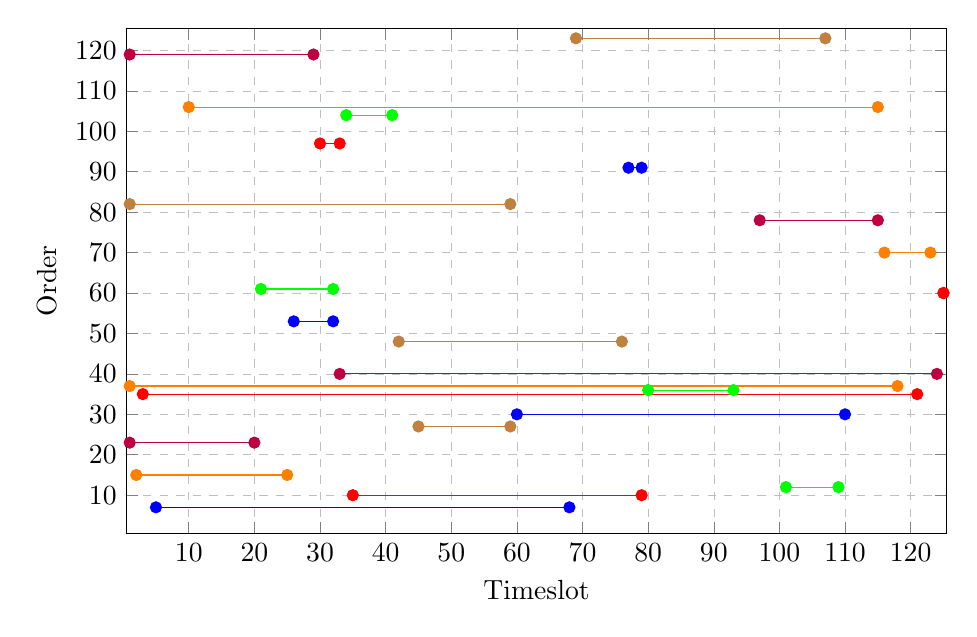
\begin{tikzpicture}
\begin{axis}[
   % title={Optimal Schedule},
    xlabel={Timeslot},
    ylabel={Order},
    xmin=0.5, xmax=125.5, 
    ymin=0.5, ymax=125.5, 
    xtick={10,20,30,40,50,60,70,80,90,100, 110, 120},
    ytick={10,20,30,40,50,60,70,80,90,100, 110, 120},
    grid=both,
    grid style={line width=.1pt, draw=gray!10},
    major grid style={line width=.2pt, draw=gray!50},
    legend pos=north east,
    ymajorgrids=true,
    xmajorgrids=true,
    grid style=dashed,
    width=12cm,
    height=8cm,
]
\addplot[color=blue, mark=*] coordinates {(5, 7) (68, 7)};
\addplot[color=red, mark=*] coordinates {(35, 10) (79, 10)};
\addplot[color=green, mark=*] coordinates {(101, 12) (109, 12)};
\addplot[color=orange, mark=*] coordinates {(2, 15) (25, 15)};
\addplot[color=purple, mark=*] coordinates {(1, 23) (20, 23)};
\addplot[color=brown, mark=*] coordinates {(45, 27) (59, 27)};
\addplot[color=blue, mark=*] coordinates {(60, 30) (110, 30)};
\addplot[color=red, mark=*] coordinates {(3, 35) (121, 35)};
\addplot[color=green, mark=*] coordinates {(80, 36) (93, 36)};
\addplot[color=orange, mark=*] coordinates {(1, 37) (118, 37)};
\addplot[color=purple, mark=*] coordinates {(33, 40) (124, 40)};
\addplot[color=brown, mark=*] coordinates {(42, 48) (76, 48)};
\addplot[color=blue, mark=*] coordinates {(26, 53) (32, 53)};
\addplot[color=red, mark=*] coordinates {(125, 60) (125, 60)};
\addplot[color=green, mark=*] coordinates {(21, 61) (32, 61)};
\addplot[color=orange, mark=*] coordinates {(116, 70) (123, 70)};
\addplot[color=purple, mark=*] coordinates {(97, 78) (115, 78)};
\addplot[color=brown, mark=*] coordinates {(1, 82) (59, 82)};
\addplot[color=blue, mark=*] coordinates {(77, 91) (79, 91)};
\addplot[color=red, mark=*] coordinates {(30, 97) (33, 97)};
\addplot[color=green, mark=*] coordinates {(34, 104) (41, 104)};
\addplot[color=orange, mark=*] coordinates {(10, 106) (115, 106)};
\addplot[color=purple, mark=*] coordinates {(1, 119) (29, 119)};
\addplot[color=brown, mark=*] coordinates {(69, 123) (107, 123)};

\end{axis}
\end{tikzpicture}
\end{figure}  
\end{frame}

\begin{frame}{Greedy cost function}
\begin{block}{Greedy cost function is split into two parts:}
    
\begin{itemize}
    \item For an order $i$:
         Only consider its profit.

    \item For a possible starting time slot $j$ (for a fixed order $i$): 
        The average percentage of space used during the baking
        \begin{center}
            $$\frac{\sum_{l=j}^{j + \mathit{length}_i} (\sum_{k=1}^n y_{kj} \mathit{surface}_k / \mathit{surface\_capacity})}{\mathit{length}_i}$$
        \end{center}
    \end{itemize}
    \end{block}
    \begin{itemize}
            \item Objective function value: 97
    \item \textbf{Optimality gap: 41\%}
    \end{itemize}
    \end{frame}

\begin{frame}{Greedy only considering profit}
%%% Greedy 97, 125_plot.dat, profit only
\begin{figure}[H]
\centering
%%% Greedy 97, 125_plot.dat, profit only
%%% E.g. order 14. altough it has a profit of 10 which is above average, it takes 114 timelots and occupies 3 slots for the basically the whole schedule. Altough they have a bit less profit, there are many orders which only take 3 surface and are way shorter to process 
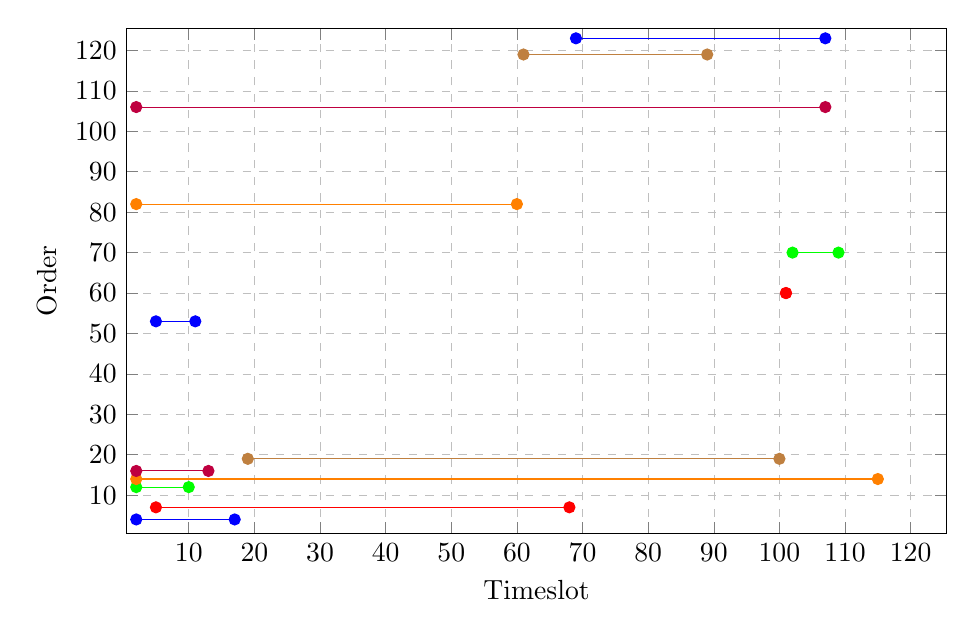
\begin{tikzpicture}
\begin{axis}[
    xlabel={Timeslot},
    ylabel={Order},
    xmin=0.5, xmax=125.5, 
    ymin=0.5, ymax=125.5, 
    xtick={10,20,30,40,50,60,70,80,90,100, 110, 120},
    ytick={10,20,30,40,50,60,70,80,90,100, 110, 120},
    grid=both,
    grid style={line width=.1pt, draw=gray!10},
    major grid style={line width=.2pt, draw=gray!50},
    legend pos=north east,
    ymajorgrids=true,
    xmajorgrids=true,
    grid style=dashed,
     width=12cm,
     height=8cm,
]
\addplot[color=blue, mark=*] coordinates {(2, 4) (17, 4)};
\addplot[color=red, mark=*] coordinates {(5, 7) (68, 7)};
\addplot[color=green, mark=*] coordinates {(2, 12) (10, 12)};
\addplot[color=orange, mark=*] coordinates {(2, 14) (115, 14)};
\addplot[color=purple, mark=*] coordinates {(2, 16) (13, 16)};
\addplot[color=brown, mark=*] coordinates {(19, 19) (100, 19)};
\addplot[color=blue, mark=*] coordinates {(5, 53) (11, 53)};
\addplot[color=red, mark=*] coordinates {(101, 60) (101, 60)};
\addplot[color=green, mark=*] coordinates {(102, 70) (109, 70)};
\addplot[color=orange, mark=*] coordinates {(2, 82) (60, 82)};
\addplot[color=purple, mark=*] coordinates {(2, 106) (107, 106)};
\addplot[color=brown, mark=*] coordinates {(61, 119) (89, 119)};
\addplot[color=blue, mark=*] coordinates {(69, 123) (107, 123)};
\end{axis}
\end{tikzpicture}

\end{figure}  
\end{frame}
    
\begin{frame}{Greedy cost function}
\begin{block}{Improvement for greedy}
For an order $i$:
        \begin{itemize}
            \item Also consider other attributes:
            $$\frac{\mathit{profit}_i (\mathit{max\_deliver}_i - \mathit{min\_deliver}_i)}{(\mathit{length}_i \cdot \mathit{surface}_i)}$$
        \end{itemize}
\end{block}

\begin{itemize}
        \item Objective function value: 126 
        \item \textbf{Optimality gap: 23\%} 
        \end{itemize}
\end{frame}

%%% Greedy 126, 125_plot.dat,         return (self.profit * (self.max_deliver - self.min_deliver)) / (self.length * self.surface)
%%% Dropped order 14 in favor of many small orders
\begin{frame}{Scoring the orders}
\begin{figure}[H]
\centering
%%% Greedy 126, 125_plot.dat,         return (self.profit * (self.max_deliver - self.min_deliver)) / (self.length * self.surface)
%%% Dropped order 14 in favor of many small orders
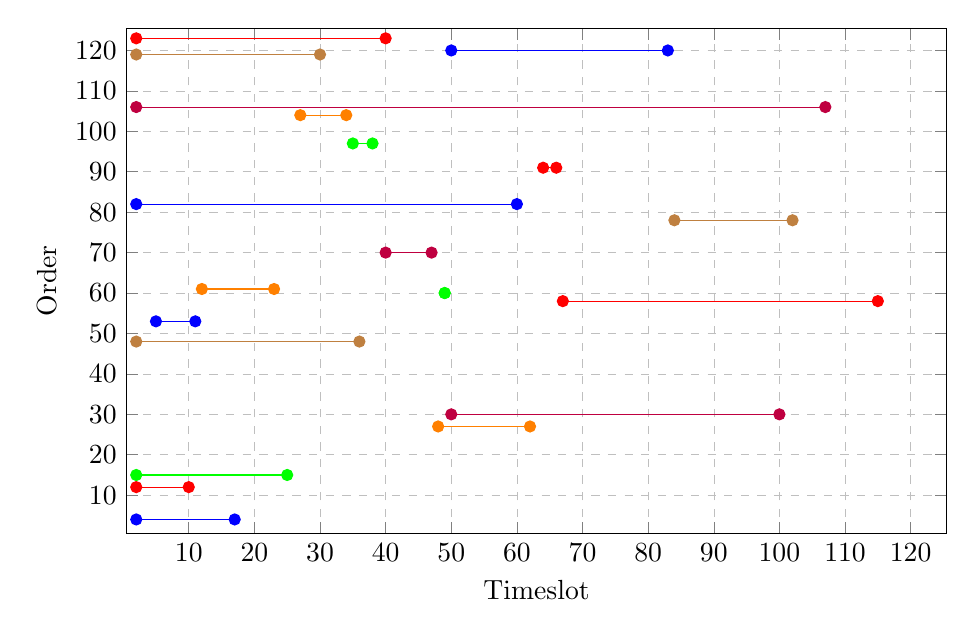
\begin{tikzpicture}
\begin{axis}[
    xlabel={Timeslot},
    ylabel={Order},
    xmin=0.5, xmax=125.5, 
    ymin=0.5, ymax=125.5, 
    xtick={10,20,30,40,50,60,70,80,90,100, 110, 120},
    ytick={10,20,30,40,50,60,70,80,90,100, 110, 120},
    grid=both,
    grid style={line width=.1pt, draw=gray!10},
    major grid style={line width=.2pt, draw=gray!50},
    legend pos=north east,
    ymajorgrids=true,
    xmajorgrids=true,
    grid style=dashed,
     width=12cm,
     height=8cm,
]
\addplot[color=blue, mark=*] coordinates {(2, 4) (17, 4)};
\addplot[color=red, mark=*] coordinates {(2, 12) (10, 12)};
\addplot[color=green, mark=*] coordinates {(2, 15) (25, 15)};
\addplot[color=orange, mark=*] coordinates {(48, 27) (62, 27)};
\addplot[color=purple, mark=*] coordinates {(50, 30) (100, 30)};
\addplot[color=brown, mark=*] coordinates {(2, 48) (36, 48)};
\addplot[color=blue, mark=*] coordinates {(5, 53) (11, 53)};
\addplot[color=red, mark=*] coordinates {(67, 58) (115, 58)};
\addplot[color=green, mark=*] coordinates {(49, 60) (49, 60)};
\addplot[color=orange, mark=*] coordinates {(12, 61) (23, 61)};
\addplot[color=purple, mark=*] coordinates {(40, 70) (47, 70)};
\addplot[color=brown, mark=*] coordinates {(84, 78) (102, 78)};
\addplot[color=blue, mark=*] coordinates {(2, 82) (60, 82)};
\addplot[color=red, mark=*] coordinates {(64, 91) (66, 91)};
\addplot[color=green, mark=*] coordinates {(35, 97) (38, 97)};
\addplot[color=orange, mark=*] coordinates {(27, 104) (34, 104)};
\addplot[color=purple, mark=*] coordinates {(2, 106) (107, 106)};
\addplot[color=brown, mark=*] coordinates {(2, 119) (30, 119)};
\addplot[color=blue, mark=*] coordinates {(50, 120) (83, 120)};
\addplot[color=red, mark=*] coordinates {(2, 123) (40, 123)};
\end{axis}
\end{tikzpicture}
\end{figure}  
\end{frame}


\begin{frame}{Local search criteria}
\begin{block}{Local Search}
    \begin{itemize} 
    \item Remove the order with the highest surface from the current schedule.
    \item Try to fit in the previously unused orders (in order of descending profit). 
    \end{itemize}
    \end{block}

    \begin{itemize} 
    \item 45 seconds of local search
    \item Objective value: 127
    \item \textbf{Optimality gap: 22.5\%}
    \end{itemize}
\end{frame}

\begin{frame}{Greedy cost function}
    \begin{block}{GRASP}
    \begin{itemize}
    \item Best results: select orders the same way as in greedy, according to their greedy cost function.
    \item Use an RCL with parameter $\alpha$ for selecting the time slot.
\end{itemize}
\end{block}

    \begin{itemize}
    \item 60 seconds, $\alpha$ = 0.8
    \item Objective value: 146
    \item \textbf{Optimality gap: 11\%}
\end{itemize}

\end{frame}

%%% GRASP, a=0.8, obj= 1min, 5 iterations, 146 obj
\begin{frame}{GRASP after 1 minute and 5 improvements}
\begin{figure}[H]
\centering
%%% GRASP, a=0.8, obj= 5min, 5 iterations, 
% Profit = 146
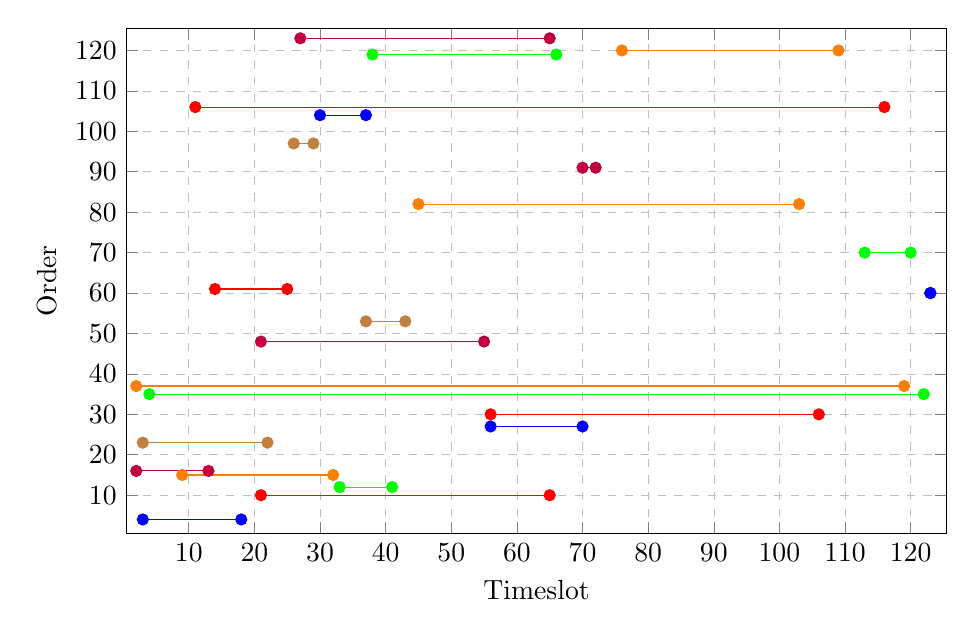
\begin{tikzpicture}
\begin{axis}[
    xlabel={Timeslot},
    ylabel={Order},
    xmin=0.5, xmax=125.5, 
    ymin=0.5, ymax=125.5, 
    xtick={10,20,30,40,50,60,70,80,90,100, 110, 120},
    ytick={10,20,30,40,50,60,70,80,90,100, 110, 120},
    grid=both,
    grid style={line width=.1pt, draw=gray!10},
    major grid style={line width=.2pt, draw=gray!50},
    legend pos=north east,
    ymajorgrids=true,
    xmajorgrids=true,
    grid style=dashed,
     width=12cm,
     height=8cm,
]
\addplot[color=blue, mark=*] coordinates {(3, 4) (18, 4)};
\addplot[color=red, mark=*] coordinates {(21, 10) (65, 10)};
\addplot[color=green, mark=*] coordinates {(33, 12) (41, 12)};
\addplot[color=orange, mark=*] coordinates {(9, 15) (32, 15)};
\addplot[color=purple, mark=*] coordinates {(2, 16) (13, 16)};
\addplot[color=brown, mark=*] coordinates {(3, 23) (22, 23)};
\addplot[color=blue, mark=*] coordinates {(56, 27) (70, 27)};
\addplot[color=red, mark=*] coordinates {(56, 30) (106, 30)};
\addplot[color=green, mark=*] coordinates {(4, 35) (122, 35)};
\addplot[color=orange, mark=*] coordinates {(2, 37) (119, 37)};
\addplot[color=purple, mark=*] coordinates {(21, 48) (55, 48)};
\addplot[color=brown, mark=*] coordinates {(37, 53) (43, 53)};
\addplot[color=blue, mark=*] coordinates {(123, 60) (123, 60)};
\addplot[color=red, mark=*] coordinates {(14, 61) (25, 61)};
\addplot[color=green, mark=*] coordinates {(113, 70) (120, 70)};
\addplot[color=orange, mark=*] coordinates {(45, 82) (103, 82)};
\addplot[color=purple, mark=*] coordinates {(70, 91) (72, 91)};
\addplot[color=brown, mark=*] coordinates {(26, 97) (29, 97)};
\addplot[color=blue, mark=*] coordinates {(30, 104) (37, 104)};
\addplot[color=red, mark=*] coordinates {(11, 106) (116, 106)};
\addplot[color=green, mark=*] coordinates {(38, 119) (66, 119)};
\addplot[color=orange, mark=*] coordinates {(76, 120) (109, 120)};
\addplot[color=purple, mark=*] coordinates {(27, 123) (65, 123)};
\end{axis}
\end{tikzpicture}
\end{figure}  
\end{frame}

%%% tuning alpha 
\begin{frame}{Tuning the $\alpha$-parameter}
\begin{figure}[H]
\centering
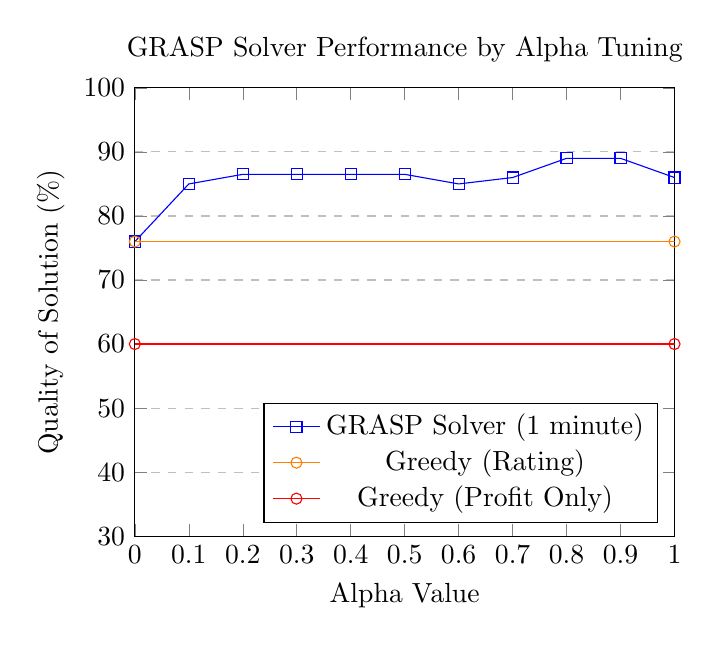
\begin{tikzpicture}
\begin{axis}[
    title={GRASP Solver Performance by Alpha Tuning},
    xlabel={Alpha Value},
    ylabel={Quality of Solution (\%)},
    xmin=0, xmax=1,
    ymin=30, ymax=100,
    xtick={0,0.1,0.2,0.3,0.4,0.5,0.6,0.7,0.8,0.9,1},
    ytick={30,40,50,60,70,80,90,100},
    legend pos=south east,
    ymajorgrids=true,
    grid style=dashed,
]

%Grasp, max obj = 146, 164, cplex
\addplot[color=blue, mark=square] coordinates {
    (0, 76) 
    (0.1, 85) % 140, 153 it
    (0.2, 86.5) % 141, 161 it
    (0.3, 86.5) % 142, 146 it 
    (0.4, 86.5) % 142 142 it
    (0.5, 86.5) % 140 157 it
    (0.6, 85) % 140 147 it
    (0.7, 86) % 141 160 it
    (0.8, 89) % 142 161 it
    (0.9, 89) % 146 150 it
    (1, 86)   % 141 149
};
\addlegendentry{GRASP Solver (1 minute)}

% Baseline solution (greedy), 126
\addplot[color=orange, mark=o] coordinates {
    (0, 76) 
    (1, 76)
};
\addlegendentry{Greedy (Rating)}
% Baseline solution (greed, profit onlyy), 97
\addplot[color=red, mark=o] coordinates {
    (0, 60) 
    (1, 60)
};
\addlegendentry{Greedy (Profit Only)}

\end{axis}
\end{tikzpicture}
%% Isert 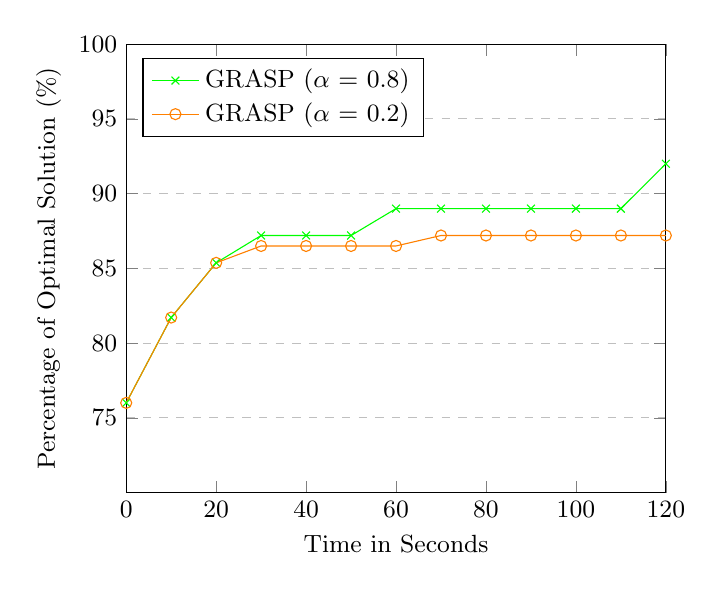
\begin{tikzpicture}
\begin{axis}[
    xlabel={Time in Seconds},
    ylabel={Percentage of Optimal Solution (\%}),
    xmin=0, xmax=120,
    ymin=70, ymax=100, % Adjusted y-axis range to fit percentage values
    xtick={0,20,40,60,80,100,120},
    ytick={75,80,85,90,95,100},
    legend pos=north west,
    ymajorgrids=true,
    grid style=dashed,
]
\addplot[color=green, mark=x] coordinates {
    (0, 76.0)
    (10, 81.71)
    (20, 85.37)
    (30, 87.20)
    (40, 87.20)
    (50, 87.20)
    (60, 89)
    (70, 89)
    (80, 89)
    (90, 89)
    (100, 89)
    (110, 89)
    (120, 92)
};
\small\addlegendentry{GRASP ($\alpha$ = 0.8)}

\addplot[color=orange, mark=o] coordinates {
    (0, 76.0)
    (10, 81.71)
    (20, 85.37)
    (30, 86.5)
    (40, 86.5)
    (50, 86.5)
    (60, 86.5)
    (70, 87.20)
    (80, 87.20)
    (90, 87.20)
    (100, 87.20)
    (110, 87.20)
    (120, 87.20)
};
\small\addlegendentry{GRASP ($\alpha$ = 0.2)}
\end{axis}
\end{tikzpicture}

\end{figure}  
\end{frame}

%%% tuning alpha 
\begin{frame}{Time and $\alpha$-parameter}
\begin{figure}[H]
\centering
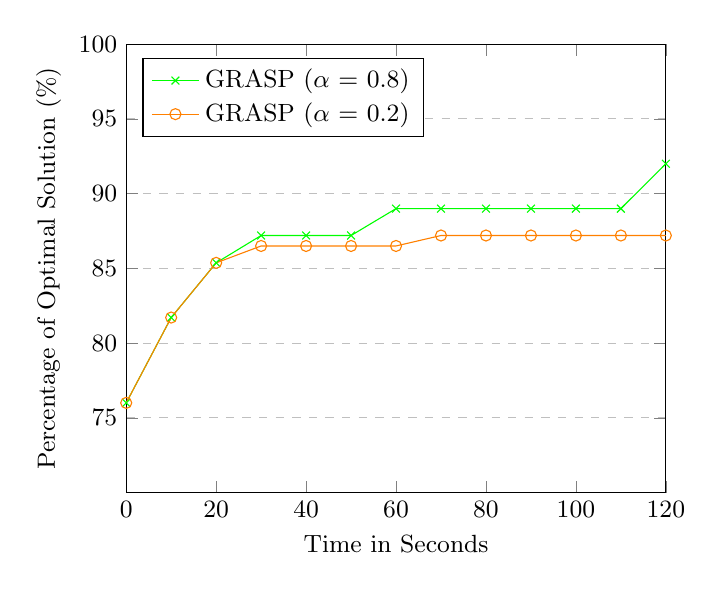
\begin{tikzpicture}
\begin{axis}[
    xlabel={Time in Seconds},
    ylabel={Percentage of Optimal Solution (\%}),
    xmin=0, xmax=120,
    ymin=70, ymax=100, % Adjusted y-axis range to fit percentage values
    xtick={0,20,40,60,80,100,120},
    ytick={75,80,85,90,95,100},
    legend pos=north west,
    ymajorgrids=true,
    grid style=dashed,
]
\addplot[color=green, mark=x] coordinates {
    (0, 76.0)
    (10, 81.71)
    (20, 85.37)
    (30, 87.20)
    (40, 87.20)
    (50, 87.20)
    (60, 89)
    (70, 89)
    (80, 89)
    (90, 89)
    (100, 89)
    (110, 89)
    (120, 92)
};
\small\addlegendentry{GRASP ($\alpha$ = 0.8)}

\addplot[color=orange, mark=o] coordinates {
    (0, 76.0)
    (10, 81.71)
    (20, 85.37)
    (30, 86.5)
    (40, 86.5)
    (50, 86.5)
    (60, 86.5)
    (70, 87.20)
    (80, 87.20)
    (90, 87.20)
    (100, 87.20)
    (110, 87.20)
    (120, 87.20)
};
\small\addlegendentry{GRASP ($\alpha$ = 0.2)}
\end{axis}
\end{tikzpicture}

\end{figure}  
\end{frame}

% TODO Discuss if we include this
% neeee
% \begin{frame}{Problem size vs. execution time}
% 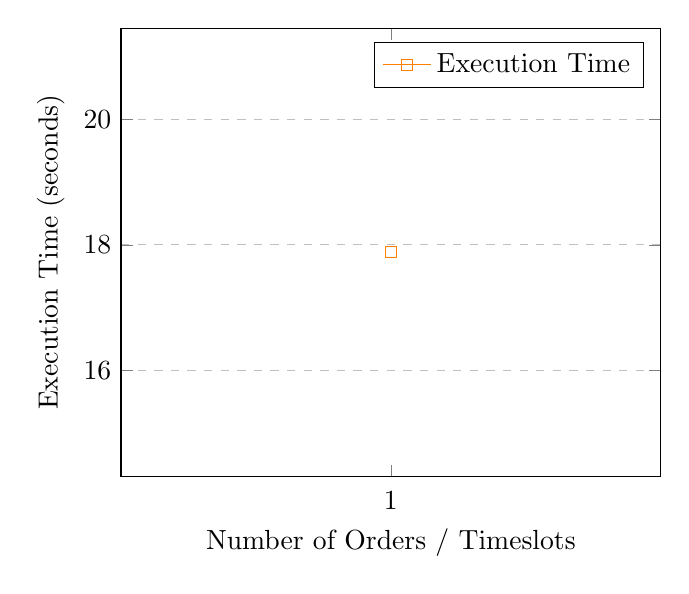
\begin{tikzpicture}
\begin{axis}[
    title={},
    xlabel={Number of Orders / Timeslots},
    ylabel={Execution Time (seconds)},
    xtick=data,
    xticklabels={1,2,4,8,16},
    symbolic x coords={1,2,4,8,16},
    xticklabel style={anchor=base, yshift=-\baselineskip},
    yticklabel style={/pgf/number format/fixed},
    legend pos=north east,
    ymajorgrids=true,
    grid style=dashed,
]
\addplot[
    color=orange,
    mark=square,
    ]
    coordinates { % 
    (1, 17.88) % Added data 8.dez
    };
    \legend{Execution Time}

\end{axis}
\end{tikzpicture}
% \end{frame}

\begin{frame}{Problem size vs. solution quality}
\centering
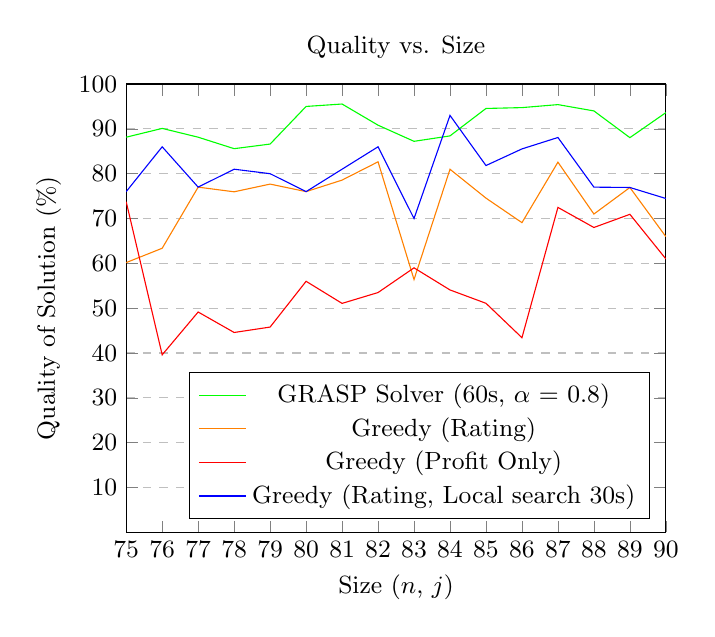
\begin{tikzpicture}
\begin{axis}[
    title={Quality vs. Size},
    xlabel={Size ($n$, $j$)},
    ylabel={Quality of Solution (\%)},
    xmin=75, xmax=90,
    ymin=0, ymax=100,
    xtick={75,76,77,78,79,80,81,82,83,84,85,86,87,88,89, 90},
    ytick={10, 20, 30, 40,50,60,70,80,90,100},
    legend pos=south east,
    ymajorgrids=true,
    grid style=dashed,
    %legend style={at={(1.05,1)},anchor=north west}
]

% GRASP Solver (1 minutes)
\addplot[color=green] coordinates {
    (75, 88.14)
    (76, 90.10)
    (77, 88.14)
    (78, 85.58)
    (79, 86.61)
    (80, 95)
    (81, 95.54)
    (82, 90.82)
    (83, 87.22)
    (84, 88.43)
    (85, 94.55)
    (86, 94.74)
    (87, 95.41)
    (88, 94)
    (89, 88.04)
    (90, 93.62)
};
\small\addlegendentry{GRASP Solver (60s, $\alpha$ = 0.8)}

% Greedy (Rating)
\addplot[color=orange] coordinates {
    (75, 60.17)
    (76, 63.37)
    (77, 77.00)
    (78, 75.96)
    (79, 77.68)
    (80, 76)
    (81, 78.57)
    (82, 82.65)
    (83, 56.39)
    (84, 80.99)
    (85, 74.55)
    (86, 69.08)
    (87, 82.57)
    (88, 71)
    (89, 76.92)
    (90, 65.96)
};
\addlegendentry{Greedy (Rating)}

% Greedy (Profit Only)
\addplot[color=red] coordinates {
    (75, 73.73)
    (76, 39.60)
    (77, 49.15)
    (78, 44.58)
    (79, 45.79)
    (80, 56)
    (81, 51.07)
    (82, 53.49)
    (83, 59.0)
    (84, 54.07)
    (85, 51.09)
    (86, 43.42)
    (87, 72.48)
    (88, 68)
    (89, 70.94)
    (90, 60.99)
};
% (75, 73.73)
%     (76, 39.60)
%     (77, 49.15)
%     (78, 35.58)
%     (79, 26.79)
%     (80, 51)
%     (81, 41.07)
%     (82, 74.49)
%     (83, 60.90)
%     (84, 52.07)
%     (85, 29.09)
%     (86, 43.42)
%     (87, 72.48)
%     (88, 68)
%     (89, 70.94)
%     (90, 60.99)
% };
\addlegendentry{Greedy (Profit Only)}

% Greedy with localsearch
\addplot[color=blue] coordinates {
    (75, 76)
    (76, 86)
    (77, 77)
    (78, 81)
    (79, 80)
    (80, 76)
    (81, 81)
    (82, 86)
    (83, 70)
    (84, 93)
    (85, 81.8181818181818)
    (86, 85.5263157894737)
    (87, 88.0733944954128)
    (88, 77)
    (89, 76.9230769230769)
    (90, 74.468085106383)
};
\addlegendentry{Greedy (Rating, Local search 30s)}


\end{axis}
\end{tikzpicture}

%%% With symbols
% % GRASP Solver (5 minutes)
% \addplot[color=blue, mark=square] coordinates {
%     (75, 88.14)
%     (76, 90.10)
%     (77, 88.14)
%     (78, 85.58)
%     (79, 86.61)
%     (80, 95)
%     (81, 95.54)
%     (82, 90.82)
%     (83, 87.22)
%     (84, 88.43)
%     (85, 94.55)
%     (86, 94.74)
%     (87, 95.41)
%     (88, 94)
%     (89, 88.04)
%     (90, 93.62)
% };
% \addlegendentry{GRASP Solver (5 minutes)}

% % Greedy (Rating)
% \addplot[color=orange, mark=o] coordinates {
%     (75, 60.17)
%     (76, 63.37)
%     (77, 77.97)
%     (78, 75.96)
%     (79, 77.68)
%     (80, 76)
%     (81, 78.57)
%     (82, 82.65)
%     (83, 56.39)
%     (84, 80.99)
%     (85, 74.55)
%     (86, 69.08)
%     (87, 82.57)
%     (88, 71)
%     (89, 76.92)
%     (90, 65.96)
% };
% \addlegendentry{Greedy (Rating)}

% % Greedy (Profit Only)
% \addplot[color=red, mark=o] coordinates {
%     (75, 73.73)
%     (76, 39.60)
%     (77, 49.15)
%     (78, 35.58)
%     (79, 26.79)
%     (80, 51)
%     (81, 41.07)
%     (82, 74.49)
%     (83, 60.90)
%     (84, 52.07)
%     (85, 29.09)
%     (86, 43.42)
%     (87, 72.48)
%     (88, 68)
%     (89, 70.94)
%     (90, 60.99)
% };
% \addlegendentry{Greedy (Profit Only)}

% % Greedy with localsearch
% \addplot[color=green, mark=square] coordinates {
%     (75, 76)
%     (76, 86)
%     (77, 77)
%     (78, 81)
%     (79, 80)
%     (80, 76)
%     (81, 81)
%     (82, 86)
%     (83, 70)
%     (84, 93)
%     (85, 81.8181818181818)
%     (86, 85.5263157894737)
%     (87, 88.0733944954128)
%     (88, 77)
%     (89, 76.9230769230769)
%     (90, 74.468085106383)
% };
% \addlegendentry{Greedy (Rating, Localsearch 45s)}
\end{frame}

\begin{frame}{Greedy and very big instances}
\centering
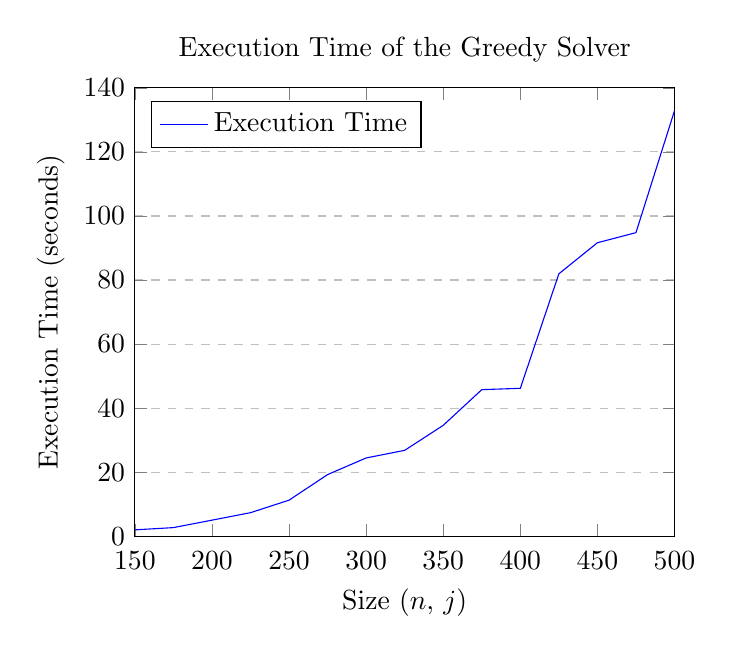
\begin{tikzpicture}
\begin{axis}[
    title={Execution Time of the Greedy Solver},
    xlabel={Size ($n$, $j$)},
    ylabel={Execution Time (seconds)},
    xmin=150, % Set minimum x value to 150
    xmax=500, % Set maximum x value
    xtick={150,200,250,300,350,400,450,500},
    xticklabels={150,200,250,300,350,400,450,500},
    ymin=0, % Set minimum y value to 0
    ymax=140, % Set maximum y value
    ytick={0,20,40,60,80,100,120,140}, % Set y ticks in steps of 20
    symbolic x coords={150,175,200,225,250,275,300,325,350,375,400,425,450,475,500},
    xticklabel style={anchor=base, yshift=-\baselineskip},
    yticklabel style={/pgf/number format/fixed},
    legend pos=north west,
    ymajorgrids=true,
    grid style=dashed,
]
\addplot[
    color=blue,
    ]
    coordinates { % 
    (150,1.98) (175,2.68) (200,5.01) (225,7.34) (250,11.25) (275,19.24) (300,24.43) (325,26.81) (350,34.62) (375,45.76) (400,46.18) (425,81.94) (450,91.64) (475,94.79) (500,132.87)
    };
    \legend{Execution Time}
\end{axis}
\end{tikzpicture}
\end{frame}

\begin{frame}{Conclusion and Future Prospects}

\begin{block}{Results}
    \begin{itemize}
    \item Developed the model
    \item Obtained optimal solutions using CPLEX
    \item Implemented and benchmarked different greedy cost functions
    \item Improved the greedy solutions using local search
    \item Applied the GRASP meta-heuristic
    \item Tuned $\alpha$ towards a consistent single-digit optimality gap in 60 seconds
\end{itemize}
\tikz[overlay, remember picture] \node[anchor=north east, xshift=-1cm, yshift=-1.95cm, rotate=-23] at (current page.north east) {\includegraphics[width=1.8cm]{project/figures/vecteezy_archivo-png-de-pan-largo-de-dibujos-animados_10178998.png}};
\end{block}

\begin{block}{Additional Considerations}
    \begin{itemize}
    \item Greedy: Try different combinations of order/time slot greedy cost functions.
    \item GRASP: Apply the RCL to the list of sorted orders to explore more diverse solutions.
\end{itemize}
\end{block}
\end{frame}

\begin{frame}{Conclusion and Future Prospects}
\centering\textbf{Backup Slides}
\end{frame}

\begin{frame}{Continuity \& Length Constraint}
\textbf{Problem:} Once started, an order has to be continuously processed for the needed time lots associated with it. 

\textbf{Constraint:}

If an order $i$ is part of the schedule, it is assigned the $\mathit{length}_i - 1$ contiguous time slots from $\mathit{start}_i$ to $\mathit{end}_i$:
    \begin{align}
      j &\geq \mathit{start}_i - (t+1) * (1-\mathit{geq\_start}_{ij}) \\
      \mathit{start}_i &\geq j - (t+1) * \mathit{geq\_start}_{ij} \\
      \mathit{end}_i &\geq j - (t+1) * (1-\mathit{leq\_end}_{ij}) \\
      j &\geq \mathit{end}_i - (t+1) * \mathit{leq\_end}_{ij} \\
      0 &\leq \mathit{geq\_start}_{ij} + \mathit{leq\_end}_{ij} - 2 * y_{ij}, &&(1 \leq i \leq n, \mathit{min\_start}_i \leq j \leq \mathit{max\_deliver}_i) 
   \end{align}

\end{frame}

\begin{frame}{CPLEX execution time}
\centering
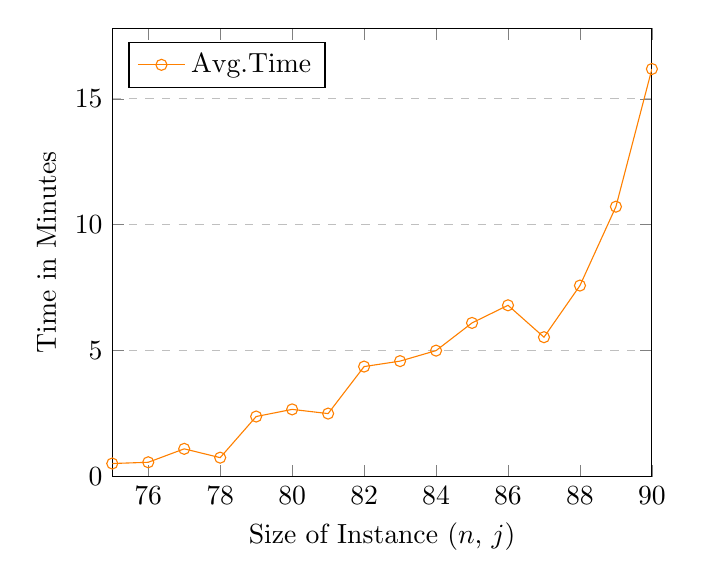
\begin{tikzpicture}
\begin{axis}[
    xlabel={Size of Instance ($n$, $j$)},
    ylabel={Time in Minutes},
    xmin=75, xmax=90,
    ymin=0, % Adjust ymin and ymax as needed
    legend pos=north west,
    ymajorgrids=true,
    grid style=dashed,
]
\addplot[color=orange, mark=o] coordinates {
    (75, 31/60)
    (76, 34/60)
    (77, 66/60)
    (78, 45/60)
    (79, 143/60)
    (80, 160/60)
    (81, 150/60)
    (82, 262/60)
    (83, 275/60)
    (84, 300/60)
    (85, 366/60)
    (86, 408/60)
    (87, 332/60)
    (88, 455/60)
    (89, 643/60)
    (90, 971/60)
};
\addlegendentry{Avg.Time}
\end{axis}
\end{tikzpicture}

\end{frame}

\end{document}

